 \subsection{Proste ścieżki na zakrzywionych powierzchniach - motywacja}

Foton poruszający się w przestrzeni kosmicznej nie jest pod wpływem zewnętrznych sił. Jest cząsteczką, na której prędkość nie wpływają zewnętrzne (ani wewnętrzne) siły, więc jego przyspieszenie przez całą podróż przez czasoprzestrzeń wokół badanej czarnej dziury pozostaje równe $0$. Z drugiej strony, nie posiada on masy, więc nie zachowuje się całkowicie jak cząsteczki materii.

Oznaczmy przez $BH$ rozmaitość opisującą czasoprzestrzeń wokół rozważanej czarnej dziury Schwarzschilda, która zazwyczaj ma postać
$$ BH = \R \times (0,+\infty) \times S^2 $$
Wówczas podróż fotonu jest opisywana przez krzywą
$$ \gamma:I \to BH $$
gdzie $I$ jest pewnym odcinkiem, a nawet może być całą prostą $\R$. Ponieważ foton porusza się z prędkością światła i nie przyśpiesza, to wiemy, że 
$$\frac{d^2 \gamma} {d t^2}=0.$$ 
Wydaje się, iż dostajemy proste równania różniczkowe opisujące zachowanie funkcji czterowymiarowej.

\renewcommand{\figurename}{Rysunek}
\begin{figure}[h] 
  \centering 
  \vspace{1cm}
  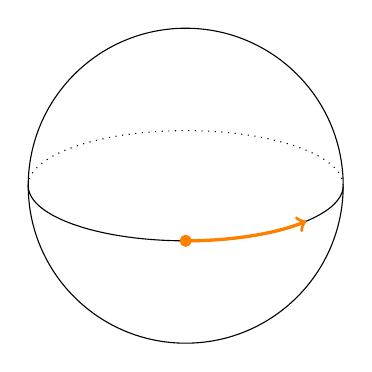
\begin{tikzpicture}
    \draw (0, 0) circle (2);
    \draw (-2, 0) arc (180:360:2 and 0.7);
    \draw[dotted] (-2, 0) arc (180:0:2 and 0.7);

    \draw[very thick, ->, orange] (0, -0.7) arc (270:320:2 and 0.7);
    \filldraw[orange] (0, -0.7) circle (2pt);
  \end{tikzpicture}
  \caption{Cząsteczka poruszająca się po sferze $S^2$.}\label{czasteczka po sferze}
  \vspace{1cm}
\end{figure}

Sprawy nie są jednak tak proste, gdyż metryka zadana na $BH$ mówi nam, że przestrzeń wokół czarnej dziury nie jest do końca taka jak przestrzeń $\R^4$. Jest ona nieco zakrzywiona i to właśnie to zakrzywienie czasoprzestrzeni będzie wpływać na obserwowane przez nas zakrzywienie trasy fotonu w pobliżu czarnej dziury. Aby zrozumieć to lepiej, wyobraźmy sobie, że foton porusza się wzdłuż równika na sferze $S^2$. Wówczas pomimo, że foton nie przyśpiesza w rozumieniu jego podróży po bardzo zagiętej przestrzeni, to dla obserwatora z zewnętrz jego prędkość cały czas się zmienia, jak na rysunku \ref{czasteczka po sferze}.

To zjawisko jest też wyrażone w tym jak różny jest produkt skalarny na badanej przez nas przestrzeni od produktu skalarnego w przestrzeni euklidesowej. Iloczyn metryczny mówi jak długi jest dany wektor, a długość krzywej jest zależna od długości wektorów, które na niej leżą. W takim razie najkrótsza droga między dwoma punktami, czyli droga z zerową drugą pochodną, będzie się zmieniać razem ze zmianą metryki. 

%Stąd nie zawsze prosta droga jest najkrótszą ścieżką między dwoma punktami. Nie jest trudno zauważyć, że tensor metryczny na jednostkowej sferze $S^2$ przedstawia się macierzą
%$$ g_(mu, nu) = \begin{bmatrix}
%  1 & 0\\
%  0 & \sin^2(\theta)\\
%\end{bmatrix} $$
%lub równoważnie wzorem $ds^2 = d \theta^2 + \sin^2(\theta) d \phi^2$, który wynika z wyliczenia długości wektora powstałego zmianę kąta $\phi$ o niewielkie zaburzenie $d \phi$ oraz kąta $\theta$ o niewielkie zaburzenie $d \theta$.
%
%Wiemy już, że pomimo braku przyśpieszenia na zakrzywionej czasoprzestrzeni wokół dziury foton będzie sprawiał wrażenie skręcającego. Chcielibyśmy teraz umieć zrekonstruować jak obserwator w $\R^3$ widzi trasę fotonu w otoczeniu $BH$ mając tylko początkowe położenie i prędkość cząsteczki. 
%
